\chapter{Anhang} \label{anhang}

\section{Hardware} \label{a:hardware}
  \subsection{Laptop}
  
\begin{table}[H]
  \begin{tabular}{|l|l|}
   \hline
    Modellbezeichnung 	& Lenovo Thinkpad Edge E330 \\
   \hline
    Prozessor		& Intel(R) Core(TM) i3-3120M CPU @ 2.50 GHz \\ 
   \hline
    Arbeitsspeicher 	& 3.5 GB \\
   \hline
    Festplatte		& 80GB SSD (Intel SSDSA2M080G2GC) \\
   \hline
    Gewicht		& 1,8 kg \\
   \hline
    Webcam		& 640 x 480 Pixel  Fixfocus  (intern)\\
                        & 16 FPS (im Dunkeln) \\
    			& FOV: $46.7^\circ \times 35.8^\circ$\\
   \hline
    Bildschirm		& 1366 x 768 Pixel 13\" TN-Panel \\
                        & LED-Backlight \\
    			& 293.5 x 165 mm \\
    \hline 
  \end{tabular} 
  \caption[Technische Daten des Laptops]{Technische Daten des Laptops.}

  \label{tab:laptop}
\end{table}

  \subsection{DSLR-Kamera}

\begin{table}[H]
  \begin{tabular}{|l|l|}
%   \hline
%    \textbf{Laptop} & \\
   \hline
    Modellbezeichnung 	& Canon EOS 5D Mark II \\
   \hline
    Sensor		& 21 MP (5616 x 3744) \\
    			& Full frame (36 x 24 mm) \\
    			& Typ: CMOS \\
   \hline
    Objektiv		& Canon EF 24-70mm f/2.8L \\
    \hline 
  \end{tabular} 
  \caption[Technische Daten der DSLR-Kamera]{Technische Daten der DSLR-Kamera}

  \label{tab:kamera}
\end{table}
\pagebreak
 \subsection{Tracking-Stage Komponenten}
  Die Komponenten des Tracking-Stage Prototyps haben  insgesamt, ohne die LED-Lampen, 35.98 
EUR gekostet und sind in der folgenden Tabelle aufgeführt. Als Werkzeug wird lediglich ein Klebestift, eine 60mm Lochsäge und eine Bohrmaschine, sowie ein Laserdrucker zum Ausdrucken der Fiducials benötigt.

 \begin{table}[H]
 \begin{tabular}{|l|l|l|}
    \hline 
    1x & Glasplatte & 50x60 cm, 2mm stark \\
   \hline
    4x & Acrylglasplatte & 15x15 cm, 2mm stark \\
   \hline
    1x & Holzkiste & 15x15x15 cm \\
   \hline
    8x & Plastikbecher & 13 hoch \\
   \hline
    1x & Blickdichter Stoff & 100x120cm \\
   \hline
    2x & Philips hue \cite{hue} LED-Lampe & \\
    \hline 
  \end{tabular} 
  \label{tab:bom}
  \caption[Komponenten der Tracking-Stage]{Die Komponenten der Tracking-Stage.}
 \end{table}



\section{Software}
   
   Der Großteil der Software, wie beispielsweise die Kalibrierungsroutinen und die Beleuchtungsberechnung, wurden in C++11 mit OpenCV  \cite{opencv} implementiert. Zur Steuerung des Framebuffers wurde OpenGL verwendet. 
   Der Toolflow  wurde mithilfe von  Shell-Skipten implementiert.
   Alle Bibliotheken und Softwarepakete, die in dieser Arbeit verwendet wurden, sind in der folgenden Tabelle aufgeführt.

  \begin{table}[H]
   \begin{tabular}{|l|l|}  
   \hline
     gcc 4.7.4 \cite{gcc}		& C++11 Compiler \\
   \hline
     OpenCV 2.4.7 \cite{opencv}		& Projektionen, Kamera-Kalibrierung, Matrixoperationen \\
   \hline
     ARToolKit 2.72.1 \cite{artoolkit}	& Marker-Tracking \\
   \hline
     gphoto2 2.5.3 \cite{gphoto2} 	& Steuerung der DSLR-Kamera \\ 
   \hline
     dcraw 9.20 \cite{dcraw} 		& Umwandlung von RAW-Formaten, De-Bayering \\ 
   \hline
     ImageMagick convert \cite{convert} &Umwandlung und Bearbeiten von (HDR)Bildern \\
   \hline
     pfstools 1.8.5 \cite{pfstools}		& Betrachten und beabeiten von HDR-Daten \\
   \hline
     pfstmo 1.5 \cite{pfstmo}		& Tone-Mapping \\
   \hline
     pfscalibration 1.5 \cite{pfscalibration}   & Rekonstruktion des Kamera-Ansprechverhaltens \\
   \hline
     OpenEXR \cite{openexr}		& Dateiformat für HDR-Daten \\
   \hline
  \end{tabular} 
  \caption[Verwendete Softwarepakete und Bibliotheken]{Verwendete Softwarepakete und Bibliotheken. }
  \label{tab:software}
 \end{table}

\section{Ergänzende Abbildungen} 
 
  \begin{figure}[H]
    \centering
    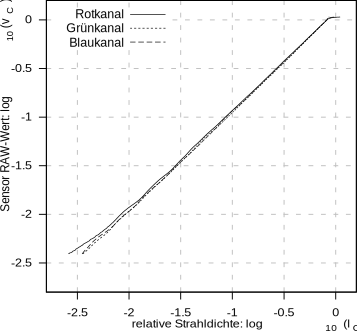
\includegraphics[width=0.65\textwidth]{../graphics/kalibrierung/canon_response_log-log.svg}
    \caption[Ansprechverhalten der DSLR im Log-Log Plot]{Doppellogarithmischer Plot des Ansprechverhalten einer Canon EOS 5D Mark II DSLR Kamera, rekonsturiert mit dem Programm pfscalibration \cite{pfscalibration}.  
    Dabei ist die relative Strahldichte $\log_{10}l_C$ über die RAW-Werte $\log_{10}v_C$ abgetragen, wobei die Messwerte auf den Bereich $(0,1)$ normiert wurden.
 }
    \label{fig:canon_response_loglog}
   \end{figure}

\begin{figure}[H]
   \centering
   
\includegraphics[width=0.55\textwidth]{../graphics/position/stage_fiducials.svg}
    \caption[Fiducials der Tracking-Stage]{Die fünf Ebenen der Tracking-Stage: Die Fiducials sind 30x30 mm groß. Die horizontale Ebene (links) besitzt insgesamt 32 Marker und misst 45x45 cm. Die vier vertikalen Ebenen (rechts) sind 15x15 cm groß, und tragen jeweils vier Fiducials. Die Marker sind farblich invertiert, da sie sich so besser zum Durchleuchten eignen.}
   \label{fig:stage_fiducials}
   \end{figure}

 \begin{figure}[H]
   $   L_{lum}(R,G,B)  = 0.212671 R +  0.71516 G + 0.072169 B $
   \caption[Formel zur Luminanzberechnung]{Formel zur Berechnung der Luminanz (aus\cite{Akenine_2011}, Seite 215 Gl. 7.11) }
  \label{eq:luminance}
 \end{figure}

 \section{Symbolverzeichnis} \label{symbolverzeichnis}
 \begin{table}[H]
  \begin{tabular}{ll}
    $(\phi,\theta)$& Polarwinkel $\phi$ und Azimuthalwinkel $\theta$ \\
    $l_{dist}(\phi,\theta)$ & Strahldichte die in einem Punkt aus Richtung  $(\phi,\theta)$ einfällt\\

  $O$ & Szenenursprung, Ursprung des Weltkoordinatensystems \\
   $r_s$ & Szenenradius \\
   $r_l$ & Lichtquellenabstand zum Ursprung $O$ \\
   $\vec{f} $ & Bildschirmzentrum im Raum\\
   $\vec{d}$ & Aufspannender Vektor der Bildschirmebene (vertikal) \\
   $\vec{r}$ & Aufspannender Vektor der Bildschirmebene (horizontal) \\
   $C$ & $3\times3$ Kamera-Matrix (intrinsische Parameter)\\
   $D$ & $3\times4$ Transformationsmatrix (extrinsische Parameter)\\

 \hline
   $L$       & Matrix: Strahldichte die jedes Pixel in einem festgelegten Punkt erzeugt\\
   $l$      & Strahldichte eines Pixels, gemessen in einem bestimmten Punkt\\
   $V$       & Framebuffer: 8 Bit, positive Ganzzahl\\
   $v$     & Framebuffer: Wert eines Pixels (8 Bit)\\
   \hline
   $l_{x,y}(v)$  &  Ansprechverhalten des Pixels mit den Koordinaten  $(x,y)$ \\
   $v_{x,y}(l)$  &  Das invertierte Ansprechverhalten des Pixels $(x,y)$ \\
   $l^0_{x,y}$  &  Kleinste Strahldichte, die von Pixel $(x,y)$ erzeugt werden kann\\
   $l^{255}_{x,y}$  &  Größte Strahldichte, die von Pixel $(x,y)$ erzeugt werden kann\\
    
   \hline
   $L_{0}$   & $L$, bei $V=0$\\
   $L_{1}$   & $L$, bei $V=1$\\
   $L_{255}$ & $L$, bei $V=255$\\
   $L'_{1}$   & $L$, bei $V=1$, wenn das Darkframe abgezogen wird\\
   $L'_{255}$ & $L$, bei $V=255$, wenn das Darkframe abgezogen wird\\
   $L_r$     & Die Strahldichte einer Teilbeleuchtung\\
   \hline
   $R$ & Dynamikbereich einer LDR-Beleuchtung \\
   $R'$ & Dynamikbereich einer LDR-Beleuchtung, bei Darkframesubtraktion \\
   $R_{HDR}$ & Dynamikbereich einer HDR-Beleuchtung \\
   \hline
   $m$   &  Länge der HDR-Sequenz\\
   $F_n$     & Pixelwerte (Framebuffer) des $n$-ten HDR-Frames\\
  % $L_{F_n}$     & Emittierte Strahldichte im $n$-ten Frame\\
   $T_i$     & Fotografierte Szene unter der $i$-ten Teilbeleuchtung\\
   $D_i$     & Darkframe der $i$-ten Teilbeleuchtung\\
   $f_i$   &  Skalierungsfaktor der  $i$-ten Aufnahme\\
   \hline
   $M$ & Alpha-Maske zum erzeugen der linearen Rampen am Bildschirmrand \\
   $E$ & Environment-Map : Zu erzeugende Umgebungsbeleuchtung \\
   $E_M$ & Environment-Map: Markiert die erzeugte Beleuchtung \\
  % $E_i$ & Die im Schritt $i$ erzeugte Teilbeleuchtung. \\

   %\caption[Symboltabelle]{\label{symboltabelle} Symboltabelle}
  \end{tabular}
 \end{table} 


